\documentclass{beamer}
%%% ========== Package setup ==========
\usepackage{xeCJK}      % Chinese words package
\usepackage{fontspec}   % Word fonts package
\usepackage{listings}   % Wrap Figure or table package
\usepackage{wrapfig}    % Multicolumn package
\usepackage{multicol}   % Multicolumn package
\usepackage{pdflscape}  % Landscpae package

%%% ========== Slide setting ==========
%% Slide theme setup
\usetheme{CambridgeUS}
\usecolortheme{wolverine}

%% Setup chinese words encoder
\XeTeXlinebreaklocale "zh"
\XeTeXlinebreakskip = 0pt plus 1pt

%% More word fonts
\setmainfont{Times New Roman}
\renewcommand{\familydefault}{\rmdefault}
\setCJKmainfont{標楷體}

% Setting for figure and table numbering
\setbeamertemplate{caption}[numbered]

%%% ========== Title setup ==========
\date{April 18, 2022}
\title{Meeting}
\author{Po Hsun Wu}

%%% ========== Document ==========
\begin{document}
    \maketitle

    \section{Progress report}

    \begin{frame}
        \frametitle{\secname}

        \begin{itemize}
            \item Optimize neural network configuration
            \begin{itemize}
                \item[1.] Pruning
                \begin{figure}
                    \centering
                    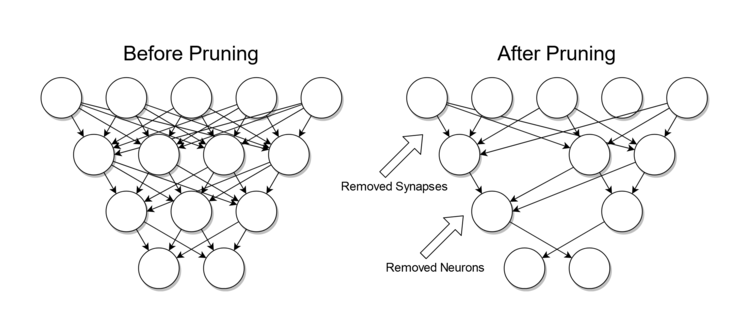
\includegraphics[scale=0.3]{Figs/Before_after_pruning.png}
                    \caption{Before and afer pruning}
                \end{figure}
            \end{itemize}
        \end{itemize}
    \end{frame}

    \section{Future}

    \begin{frame}
        \frametitle{\secname}

        \begin{itemize}
            \item Using OpenAI Gym package to complete RL problem.
        \end{itemize}

    \end{frame}

\end{document}